\begin{example}\label[example]{51e}
Let $C$ be a ringed site with no affines. 
Therefore no object can have the empty sieve as a covering sieve, because that would make all sheaves trivial restricted at this object.
Let $\sheaf{O}$ be its structure sheaf.

Let $a$ be an object of $C$.
Let $b$ be an object of $C$ such that $\Hom{b}{a}=\emptyset$.

The following situation, the commuting square with conditions on the maps and objects, will be called $S1$.
Note that $a,b$ are fixed and not variables in $S1$. 

\begin{center}
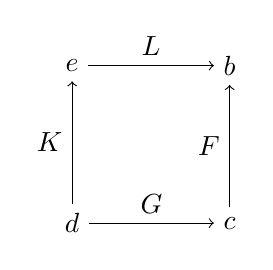
\begin{tikzpicture}[node distance=2cm, auto]
  \node (C) {$c$};
  \node (B) [above of =C] {$b$};
  \node (D) [left of =C] {$d$};
  \node (E) [above of =D] {$e$};
  \draw[->] (C) to node {$F$} (B);
  \draw[->] (D) to node {$G$} (C);
  \draw[->] (D) to node {$K$} (E);
  \draw[->] (E) to node {$L$} (B);
\end{tikzpicture}
\end{center}

With $\sheaf{O}(d)\neq 0$, $\Hom{e}{a}=\emptyset$ and $\Hom{c}{a}\neq\emptyset$ .

Assume that for any $S$ a covering sieve on $b$.

1) every map $F\in S$ as in $S1$, so $F$ has codomain $b$ and its domain maps to $a$,
we can find maps $G,K,L$ to complete to $S1$ with $L\in S$.

2) For every $L\in S$ as in $S1$, so $L$ has codomain $b$ and its domain does not map to $a$, we can complete the to get $S1$.

Consequences: Every non-empty covering sieve of $b$ contains maps $L$ and $F$ that fit in $S1$.
'Objects under $a$ get under every object under $b$'.
Call this assumption $A1$ en $A2$.

Define the presheaf $\presheaf{F}$ as

\[ x \mapsto \sheaf{O}(x) \mbox{ if } \Hom{x}{a}=\emptyset, \]
\[ x \mapsto \sheaf{O}(x)[y] \otherwise,\] 

\[ u \xrightarrow{f} v \mapsto \sheaf{O}(f) \mbox{ if } \Hom{u}{a} = \emptyset, \]
\[ u \xrightarrow{f} v \mapsto (\sheaf{O}(u) \rightarrow \sheaf{O}(u)[y]) \circ \sheaf{O}(f) 
\mbox{ if } \Hom{u}{a} \neq \emptyset \; \& \; \Hom{v}{a} = \emptyset,\]
\[ u \xrightarrow{f} v \mapsto \sheaf{O}(f) \otherwise.\]

Let $G = \presheaf{F}^{++}$.


%%show G(b) = \sheaf{O}(b)

Let $S$ be a covering sieve on $b$. If $S$ is empty, then $G(b) = 0 = \sheaf{O}(b)$.
Assume otherwise.
Let $(x_f)$ be a matching family indexed by $S$.
Let $x_f\in G(u)\setminus O(u)$ for $u\xrightarrow{f} b$ such that $\Hom{u}{a} \neq \emptyset$, 
which is possible by $A2$. Set $F=f$ and complete to $S1$. Then $\presheaf{F}(G)(x_F)= \presheaf{F}(K)(x_L) = x_{KL}$ since it is a matching family,
which is impossible because $\presheaf{F}(G)(x_F)$ is not in the image of $\presheaf{F}(K)$.
So all matching families $(x_f)$ have components that are elements of $O(\Dom{f})\subset G(\Dom{f})$, 
which already have unique amalgamations in $\sheaf{O}(b)$. 
Hence $G(b)= \sheaf{O}(b)$.

%%Show G is not quasi-coherent
Let $U$ be a global cover of the category.
By A1, $U(b)$ contains an element $g:e\rightarrow b$ with $\Hom{e}{a} = \emptyset$.
Set $g=L$ and complete $S1$.
The element $y\in G(d)$ is not generated locally by sections of $G(e)$.
Hence $G$ is not locally presentable.

\emph{Examples that satisfy A1\&A2}
\begin{itemize}
\item Open category of any irreducible space.
\item Neighbourhood space of any point in any topological space.
\item categories with pullbacks, terminal object and are irreducible.
\end{itemize}
\end{example}